\section{Nombres complexes}

Lorsque l'humanité à créer les nombres, ils étaient limités aux entiers positifs. L'humanité y a progressivement inclus des nombres négatifs, puis des nombres réels. Cependant, bien que ces nombres suffisent en général, d'autres ensemble de nombres plus larges existent également comme les \glspl{Complex-number} qui sont le sujet de ce chapitre.

\subsection{Avantages}

Bien que ces \glspl{Complex-number} étaient considérés comme une astuce pour résoudre des problèmes ayant des racines carrés de nombres négatifs, ces nombres sont désormais très souvent utilisés en mathématique, en physique et en ingénierie. Ils permettent de simplifier l'écriture de nombreuses formules et sont suffisants pour décrire une grande majorité des lois et phénomènes physiques.

Une raison majeure de la nécessité d'intégrer dans l'arsenal mathématique le corps des \glspl{Complex-number} tient au fait qu'il est algébriquement clos. C'est-à-dire que chaque polynôme complexe de degré 1 ou supérieur a au moins une racine complexe. Ainsi, il n'y a pas les mêmes risques que pour les nombres réels où chaque calcul de racine doit être fait avec précautions sans quoi, il pourrait n'exister aucune solution dans le domaine réel. Avec les \glspl{Complex-number}, il est garanti qu'une racine existera nécessairement.

Les \glspl{Complex-number} ont eux aussi des limites, même si on ne les rencontre que rarement. C'est seulement dans des cas spécifiques, tel que la physique quantique avec un spin, que les \glspl{Complex-number} se révèlent insuffisants \cite{spineurs}.

\subsection{Désavantages}

Les \glspl{Complex-number} ont aussi un désavantage: la perte de comparaison. Comme les nombres réels peuvent être représentés sur un axe, il est toujours possible de définir si un nombre est plus petit ou plus grand qu'un autre. Cette même comparaison n'a plus lieu d'être avec les \glspl{Complex-number}, car il ne s'agit plus d'un axe, mais d'un espace à 2 dimensions. Selon les situations, les \glspl{Complex-number} peuvent être comparés par leur partie réelle, par leur partie imaginaire, par leur module ("la taille" de ce nombre), etc.

\subsection{Représentations}
\label{sec:complex_representations}

Les \glspl{Complex-number} peuvent être écrits sous différentes formes:

\begin{itemize}
    \item Algébrique: $a + bi$ où $a$ est la partie réelle et $bi$ est la partie imaginaire. Ex: $3 - 2i$
    \item Trigonométrique: $r(cos(\theta) + i \cdot sin(\theta))$
    \item Exponentielle: $re^{i\theta}$
    \item Polaire: $(r, \theta)$
\end{itemize}

Voici l'exemple du nombre $3 - 2i$ visible sur la Figure \ref{fig:complex_3-2i}.

\begin{minipage}{\linewidth}
\makebox[\linewidth]{
    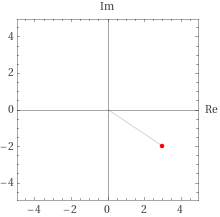
\includegraphics[width=.5\linewidth]{complex_numbers/3-2i.png}
}
\captionof{figure}{Le nombre $3 - 2i$ dans l'espace complexe}
\label{fig:complex_3-2i}
\end{minipage}

Voici les différentes notations correspondant toutes au nombre $3 - 2i$:

\begin{itemize}
    \item Algébrique: $3 - 2i$
    \item Trigonométrique: $\sqrt{13} \cdot (cos(-tan^{-1}(\frac{2}{3})) + i \cdot sin(-tan^{-1}(\frac{2}{3})))$
    \item Exponentielle: $\sqrt{13} \cdot e^{-i \cdot tan^{-1}(\frac{2}{3})}$
    \item Polaire: $(\sqrt{13}, -tan^{-1}(\frac{2}{3}))$
\end{itemize}

Dans chacune de ces formes, on connaît soit la partie réelle et la partie imaginaire, soit l'angle et le module (ou rayon) du nombre complexe. On peut passer d'une forme à l'autre en utilisant les formules de Pythagore et de trigonométrie.

Les variables suivantes seront utilisées:

\begin{itemize}
    \item Partie réelle: $a$
    \item Partie imaginaire: $b$
    \item Module/rayon: $r$
    \item Angle: $\theta$
\end{itemize}

On peut ensuite définir les conversions entre la forme cartésienne et polaire de la manière suivante:

\begin{itemize}
    \item $a = r cos(\theta)$
    \item $b = r sin(\theta)$
    \item $r = \sqrt{a^2 + b^2}$
    \item $\theta = tan^{-1}(y/x)$
\end{itemize}
